\documentclass{beamer}

\newenvironment{tightcenter}{%
  \setlength\topsep{0pt}
  \setlength\parskip{0pt}
  \begin{center}
}{%
  \end{center}
}

\mode<presentation>
{
  \usetheme{Copenhagen}
  %%\usecolortheme[RGB={173,222,25}]{structure}
  \usecolortheme[RGB={66,134,244}]{structure}
  \setbeamertemplate{items}[circle]
  \setbeamercovered{transparent}
}

\usepackage[polish]{babel}
\usepackage{chessfss}
\PassOptionsToPackage{hyphens}{url}
\usepackage{hyperref}
\usepackage{qtree}
\usepackage{mathtools}
\usepackage{dirtytalk}
\usepackage{epigraph}
\usepackage{textgreek}
\usepackage[utf8]{inputenc}
\usepackage{times}
\usepackage[T1]{fontenc}
\usepackage{tikz}
\usepackage{csquotes}
\usepackage{amsmath}
\usepackage{fancyvrb}
\usepackage{ulem}
\usepackage{adjustbox}

\newcommand{\prompt}{\phantom{}>\phantom{}>\phantom{}>\ }

\newenvironment{Snippet}{\Verbatim[samepage=true]}{\endVerbatim}

\title{\textbf{The Hassle with Monads}}

\author{Panicz Maciej Godek}

\institute{
  \tiny{\href{https://twitter.com/PaniczGodek}{\textbf{@PaniczGodek}}} \\
  \normalsize{\url{https://github.com/panicz/writings/tree/master/talks/datamass}}
}

\date{\textbf{datamass.io summit}, 28.09.2018}

\begin{document}

\begin{frame}
  \titlepage
\end{frame}

\begin{frame}{Before we begin - questions to the audience:}
  \begin{itemize} \pause
  \item do you program? \pause
  \item do you not program?
  \end{itemize}
\end{frame}

\begin{frame}{Which languages do you know?}
  \begin{itemize} \pause
  \item Java/C\# \pause
  \item Python \pause
  \item JavaScript \pause
  \item C/C++ \pause
  \item Scala \pause
  \item Erlang/Elixir \pause
  \item OCaml/F\# \pause
  \item Haskell \pause
  \item some other?
  \end{itemize}
\end{frame}

\begin{frame}{On to the topic}
  \begin{itemize} \pause
  \item do you know functional programming? \pause
  \item have you heard about monads? \pause
  \item do you understand monads? \pause
  \item did you try to understand monads and failed?
  \end{itemize}
\end{frame}


\begin{frame}{Why learn monads?}

  \begin{displayquote}
    Yes, monads seem to be a form of AspectOrientedProgramming,
    since they serve to isolate a generalized computational
    strategy from the specifics of an algorithm. For example,
    in HaskellLanguage you can write a graph-searching
    procedure that can either do a depth-first search
    and return the first result, or do a breadth-first
    search and return a list of results, merely by running
    it in a different monad.
  \end{displayquote}

  \begin{flushright}
    {\footnotesize \url{http://wiki.c2.com/?AspectOrientedProgramming}}
  \end{flushright}
  
\end{frame}

\begin{frame}{Why learn monads?}
  
\includegraphics[width=\textwidth]{hello-haskell.jpg}
\end{frame}

\begin{frame}{Why (lazy) functional programming?}
  
\includegraphics[width=\textwidth]{recursive-centaur.png}
\end{frame}

\begin{frame}{Why (lazy) functional programming?}
  \texttt{numbersFrom n = n:numbersFrom(n+1)}\\ \pause
  \texttt{numbersFrom 0 = [0,1,2,3,4,5,6,7,8,9,10,...]}\\ \pause
  \ \\
  \texttt{sieve (h:t) = h:(sieve [x|x<-t,x`mod`h/=0])} \\ \pause
  \texttt{primes = sieve (numbersFrom 2)} \\ \pause
  \texttt{primes = [2,3,5,7,11,13,17,19,23,29,31,37,...]} \\ \pause
  \ \\ \
  \\ Jerzy Karczmarczuk, \textit{Generating Power of Lazy Semantics} \\ \pause  John Hughes, \textit{Why Functional Programming Matters}
\end{frame}

\begin{frame}{The essence of laziness}
  \texttt{square x = x * x} \\ \pause
  \ \\
  Applicative order (evaluate arguments before expansion): \\ \pause
  \texttt{square (2*3) \pause = square 6 \pause =$_{def}$ 6 * 6 \pause = 36} \\ \pause
  \ \\
  Normal order (evaluate arguments after expansion): \\ \pause
  \texttt{square (2*3) \pause =$_{def}$ (2*3) * (2*3) \pause = 6 * 6 \pause = 36}
\end{frame}

\begin{frame}{Lambda the Ultimate}
  \texttt{square x = x * x} \\ \pause
  \texttt{square = λ x -> x * x} \\ \pause
  \texttt{square = function(x) \{ return x * x; \} } \\ \pause
  \ \\
  \texttt{distance x y = abs(x-y)} \\ \pause
  \texttt{distance = λ x -> λ y -> abs(x-y)} \textit{(currying)} \\ \pause
  \ \\
  \texttt{\textbf{let} name = value \textbf{in} expression} \\ \pause
  \texttt{(λ name -> expression) value}
\end{frame}

\begin{frame}{The problem with I/O}
  \texttt{1*3 + 2*0} \\ \pause
  \ \\
  \texttt{readNumber()*3 + 2*readNumber()} \\ \pause
  \texttt{\phantom{}< 1} \\
  \texttt{\phantom{}< 0} \\
\end{frame}

\begin{frame}{Attempted solution}
  \texttt{ \\ \ \\
    let \ a\ \ \ \ \  = readNumber(\ \ ) in \\ \pause
    \ \ let \ b\ \ \ \ \ = readNumber(\ \ ) in \\ \pause
    \ \ \ \ \ a*2 + 3*b
  } \\ \ \\ \ \\ \ 
\end{frame}

\begin{frame}{Actual solution}
  \texttt{ \\ \ \\
    let (a,w1) = readNumber(w0) in \\
    \ \ let (b,w2) = readNumber(w1) in \\
    \ \ \ \ \ a*2 + 3*b
  } \\ \ \\ \ \\ \ 
\end{frame}

\begin{frame}{Better (composable) solution}
  \texttt{ \\ \ \\
    let (a,w1) = readNumber(w0) in \\
    \ \ let (b,w2) = readNumber(w1) in \\
    \ \ \ \ (a*2 + 3*b, w2)
  } \\ \ \\ \ \\ \ 
\end{frame}

\begin{frame}{A function}
  \texttt{ \\
    myOperation w0 = \\
    let (a,w1) = readNumber(w0) in \\
    \ \ let (b,w2) = readNumber(w1) in \\
    \ \ \ \ (a*2 + 3*b, w2)
  } \\ \ \\ \ \\ \ 
\end{frame}

\begin{frame}{A function}
  \texttt{myOperation ::\ RealWorld -> (Int, RealWorld)
    myOperation w0 = \\
    let (a,w1) = readNumber(w0) in \\
    \ \ let (b,w2) = readNumber(w1) in \\
    \ \ \ \ (a*2 + 3*b, w2)
  } \\ \ \\ \ \\ \url{https://wiki.haskell.org/IO_inside}
\end{frame}

\begin{frame}{Downsides}
  \pause
  \begin{itemize}
  \item need to pass additional parameter \pause
  \item prone to errors (e.g. \texttt{w0} instead of \texttt{w1}) \pause
  \item nesting level increases \pause
  \end{itemize} \ \\ Could we do something to make \texttt{w0} passed implicitly?
\end{frame}


\begin{frame}{How could this look like?}
  \texttt{pass readNumber \\
    \ \ \ \ \ (λ a \pause -> pass readNumber \\
    \ \ \ \ \ \ \ \ \ \ \ \ \ \ \ \ \ \ (λ b \pause -> return a*2 + 3*b)) \\
    \ \\ \pause
    return value world = (value, world) \\ \pause
    \ \\
    pass value continuation w0 = \\
    \ \ let (result, w1) = value w0 in \\
    \ \ \ \ \ continuation result w1
  }
\end{frame}

\begin{frame}{Does this really work?}
  \texttt{pass readNumber\\
    \ \ \ \ \ (λ a -> pass readNumber\\
    \ \ \ \ \ \ \ \ \ \ \ \ \ \ \ \ \ \ (λ b -> \textbf{return a*2 + 3*b}))\\
    \ \\ \pause
    \textbf{return value world = (value, world)} \\ \pause
    \ \\
    pass value continuation w0 = \\
    \ \ let (result, w1) = value w0 in \\
    \ \ \ \ \ continuation result w1
  }
\end{frame}

\begin{frame}{Does this really work?}
  \texttt{pass readNumber\\
    \ \ \ \ \ (λ a -> pass readNumber\\
    \ \ \ \ \ \ \ \ \ \ \ \ \ \ (λ b -> \textbf{λ w -> (a*2 + 3*b, w)}))\\
    \ \\
    \textbf{return value world = (value, world)} \\
    \ \\
    pass value continuation w0 = \\
    \ \ let (result, w1) = value w0 in \\
    \ \ \ \ \ continuation result w1
  }
\end{frame}

\begin{frame}{Does this really work?}
  \texttt{pass readNumber\\
    \ \ \ \ \ (λ a -> \textbf{pass readNumber\\
      \ \ \ \ \ \ \ \ \ \ \ \ \ \ (λ b -> λ w -> (a*2 + 3*b, w))})\\
    \ \\
    return value world = (value, world) \\
    \ \\
    \textbf{pass value continuation w0 = \\
      \ \ let (result, w1) = value w0 in \\
      \ \ \ \ \ continuation result w1}
  }
\end{frame}

\begin{frame}{Does this really work?}
  \texttt{pass readNumber (λ a -> \textbf{λ w1 -> \\
      \ \ let (y, w2) = readNumber(w1) in\\
      \ \ \ \ \ \ \ \ (λ b -> λ w -> (a*2 + 3*b, w)) y w2})\\
    \ \\
    return value world = (value, world) \\
    \ \\
    \textbf{pass value continuation w0 = \\
      \ \ let (result, w1) = value w0 in \\
      \ \ \ \ \ continuation result w1}
  }
\end{frame}

\begin{frame}{Does this really work?}
  \texttt{pass readNumber (λ a -> λ w1 -> \\
    \ \ let (y, w2) = readNumber(w1) in\\
    \ \ \ \ \ \ \ \ \ \textbf{(λ b -> λ w -> (a*2 + 3*b, w)) y w2})\\
    \ \\
    return value world = (value, world) \\
    \ \\
    pass value continuation w0 = \\
    \ \ let (result, w1) = value w0 in \\
    \ \ \ \ \ continuation result w1
  }
\end{frame}

\begin{frame}{Does this really work?}
  \texttt{pass readNumber (λ a -> λ w1 -> \\
    \ \ let (y, w2) = readNumber(w1) in\\
    \ \ \ \ \ \ \ \ \ \textbf{(λ w -> (a*2 + 3*y, w)) w2})\\
    \ \\
    return value world = (value, world) \\
    \ \\
    pass value continuation w0 = \\
    \ \ let (result, w1) = value w0 in \\
    \ \ \ \ \ continuation result w1
  }
\end{frame}

\begin{frame}{Does this really work?}
  \texttt{pass readNumber (λ a -> λ w1 -> \\
    \ \ let (y, w2) = readNumber(w1) in\\
    \ \ \ \ \ \ \ \ \ \textbf{(a*2 + 3*y, w2)})\\
    \ \\
    return value world = (value, world) \\
    \ \\
    pass value continuation w0 = \\
    \ \ let (result, w1) = value w0 in \\
    \ \ \ \ \ continuation result w1
  }
\end{frame}

\begin{frame}{Does this really work?}
  \texttt{\textbf{pass readNumber (λ a -> λ w1 ->\\
      \ \ let (y, w2) = readNumber(w1) in\\
      \ \ \ \ \ \ \ \ (a*2 + 3*y, w2))}\\
    \ \\
    return value world = (value, world) \\
    \ \\
    \textbf{pass value continuation w0 = \\
      \ \ let (result, w1) = value w0 in \\
      \ \ \ \ \ continuation result w1}
  }
\end{frame}

\begin{frame}{Does this really work?}
  \texttt{\textbf{λ w0 -> let (x,w3) = readNumber(w0) in\\
      \ \ (λ a -> λ w1 -> let (y, w2) = readNumber(w1) \\
      \ \ \ \ \ \ in (a*2 + 3*y, w2)) x w3}\\
    \ \\
    return value world = (value, world) \\
    \ \\
    \textbf{pass value continuation w0 = \\
      \ \ let (result, w1) = value w0 in \\
      \ \ \ \ \ continuation result w1}
  }
\end{frame}

\begin{frame}{Does this really work?}
  \texttt{λ w0 -> let (x,w3) = readNumber(w0) in\\
    \ \ \textbf{(λ a -> λ w1 -> let (y, w2) = readNumber(w1)\\
      \ \ \ \ \ \ in (a*2 + 3*y, w2)) x w3}\\
    \ \\
    return value world = (value, world) \\
    \ \\
    pass value continuation w0 = \\
    \ \ let (result, w1) = value w0 in \\
    \ \ \ \ \ continuation result w1
  }
\end{frame}

\begin{frame}{Does this really work?}
  \texttt{λ w0 -> let (x,w3) = readNumber(w0) in\\
    \ \ \textbf{(λ w1 -> let (y, w2) = readNumber(w1) in\\
      \ \ \ \ \ \ \ \ \ (x*2 + 3*y, w2)) w3}\\
    \ \\
    return value world = (value, world) \\
    \ \\
    pass value continuation w0 = \\
    \ \ let (result, w1) = value w0 in \\
    \ \ \ \ \ continuation result w1
  }
\end{frame}

\begin{frame}{Does this really work?}
  \texttt{λ w0 -> let (x,w3) = readNumber(w0) in\\
    \ \ \textbf{let (y, w2) = readNumber(w3) in\\
      \ \ \ \ \ \ \ \ \ (x*2 + 3*y, w2)}\\
    \ \\
    return value world = (value, world) \\
    \ \\
    pass value continuation w0 = \\
    \ \ let (result, w1) = value w0 in \\
    \ \ \ \ \ continuation result w1
  }
\end{frame}

\begin{frame}{Does this really work?}
  \texttt{λ w0 -> let (x,w3) = readNumber(w0) in\\
    \ \ let (y, w2) = readNumber(w3) in\\
      \ \ \ \ \ \ \ \ \ (x*2 + 3*y, w2)\\
    \ \\ \ \\
    let (a,w1) = readNumber(w0) in \\
    \ \ let (b,w2) = readNumber(w1) in \\
    \ \ \ \ (a*2 + 3*b, w2) \\
    \ 
  }
\end{frame}


\begin{frame}{It works!}
  \texttt{pass readNumber \\
    \ \ \ \ \ (λ a -> pass readNumber \\
    \ \ \ \ \ \ \ \ \ \ \ \ \ \ \ \ \ \ (λ b -> return a*2 + 3*b))
  } \\ \ \\ \pause
  But typing λ and the increased indentation level is annoying! \\ \pause
  \ \\
  \texttt{pass readNumber (λ a \\
    -> pass readNumber (λ b \\
    -> return a*2 + 3*b))
  } 
\end{frame}

\begin{frame}
  \ \\ Introduce new syntax (\texttt{do}-notation): \\
  \texttt{
    \ \ do result <- action \\
    \ \ \ \ \ \ actions  ... \\
  } \ \\ \pause
  can be interpreted as: \\ \pause
  \texttt{
    \ \ pass action (λ result -> do actions ...) \\
  } \ \\  \pause
  \ \\
  Note: In Haskell, \texttt{pass} function is spelled
  \texttt{>>=} and pronounced ``bind''.
\end{frame}

\begin{frame}{Emperor's new clothes}
  Now we can write our program as: \\
  \texttt{ \\
    \ \ do a <- readNumber\\
    \ \ \ \ \ b <- readNumber \\
    \ \ \ \ \ return a*2 + 3*b
  }
\end{frame}

\begin{frame}{The sequencing pattern} \pause
  A monad (sequencing pattern) consists of: \pause
  \begin{enumerate}
  \item a \texttt{>>=} (bind, pass, chain) function
    that takes some (decorated) value and a function (\textit{continuation}) and
    passes that value to the function \pause
  \item a \texttt{return} function that takes some
    (raw) value and lifts (decorates) it, so that it
    can be chained using the \texttt{>>=} operator \pause
  \end{enumerate}
  \ \\ \textbf{The monad laws:} \pause
 
  \texttt{((return v) >>= f) = (f v)} \pause \textit{-- left identity} \\ \pause
  \texttt{(m >>= return) = m} \pause \textit{-- right identity}
\end{frame}

\begin{frame}{In Haskell} \pause
  \texttt{class \textbf{Monad} m where\\ \pause
    \ \ return\ ::\ a -> m a\\ \pause
    \ \ (>>=)\ ::\ m a -> (a -> m b) -> m b\\ \pause
  } \ \\
  Monads with the \texttt{do} notation provide a general
  and systematic solution to the common anti-pattern known
  as \textit{the Pyramid of Doom}.
\end{frame}

\begin{frame}{The Pyramid of Doom}
  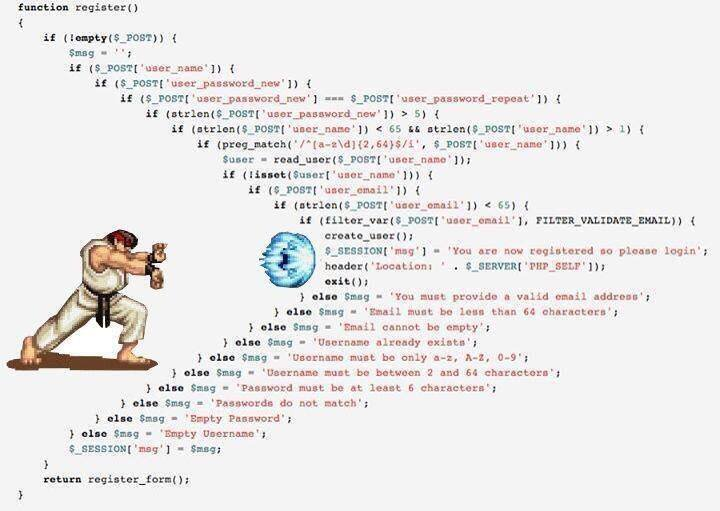
\includegraphics[width=\textwidth]{pyramid-of-doom.jpg}  
\end{frame}

\begin{frame}{The Pyramid of Doom}
  \begin{displayquote}
    In computer programming, the \textbf{pyramid of doom}
    is a common problem that arises when a program uses many
    levels of nested indentation to control access to a function.
    It is commonly seen when checking for null pointers or handling
    callbacks.
  \end{displayquote}
  
  \begin{flushright}
    {\footnotesize \href{https://en.wikipedia.org/wiki/Pyramid_of_doom_(programming)}{Wikipedia/Pyramid\_of\_doom\_(programming)}}
  \end{flushright}
\end{frame}

\begin{frame}{The Pyramid of Doom -- example} \pause
  {\footnotesize
    \texttt{theWidth = windows(``Main'').views(5).size().width();} \\ \pause
    \ \\
    \texttt{if windows.contains(``Main'') \{ \\
      \ \ if windows(``Main'').views.contains(5) \{ \\
      \ \ \ \ theWidth = windows(``Main'').views(5).size().width();\\
      \ \ \ \ //more code that works with theWidth\\
      \ \ \}\\
      \}\\
    } \pause
    \ \\
    With ``optional chaining''/``null-conditional''/``safe navigation''
    operator: \\ \pause
    \texttt{theWidth = windows(``Main'')?.views(5)?.size.width;}
  }
\end{frame}

\begin{frame}{Dealing with ``no values'' in Haskell} \pause
  \texttt{data Maybe a = Nothing | Just a} \\ \pause
  \ \\
  \texttt{let theWidth = do window <- windows(``Main'')\\
    \ \ \ \ \ \ \ \ \ \ \ \ \ \ \ \ \ \ view <- views 5 window\\
    \ \ \ \ \ \ \ \ \ \ \ \ \ \ \ \ \ \ return width (size view)\\
  } \ \\ \pause
  
  \texttt{instance Monad Maybe where\\ \pause
    \ \ (Nothing >>= f) = Nothing\\ \pause
    \ \ (Just a >>= f) = (f a)\\ \pause
    \ \ return a = Just a}
\end{frame}

\begin{frame}{The List Monad}
  \texttt{instance Monad List where\\ \pause
    \ \ (x >>= f) = concatMap f x \\ \pause
    \ \ return a = [a] \\ \pause
  } \ \\
  \texttt{\prompt{} concatMap (λ n -> [1..n]) [1,2,3]} \\ \pause
  \texttt{ [1, 1,2, 1,2,3] } \\ \ \\ \pause
  \texttt{\prompt{} do a <- [1,2,3] \\
    \ \ \ \ \ \ \ \ b <- [4,5] \\
    \ \ \ \ \ \ \ \ return (a, b)} \\ \pause
  \ \\
  \texttt{[(1,4),(1,5),(2,4),(2,5),(3,4),(3,5)]}
\end{frame}

\begin{frame}{The Amb Monad} \pause
  \texttt{import Control.Monad \\
    import Control.Monad.Amb \\
    \ \\
    pyTriple n = do a <- anIntegerBetween 1 n \\
    \ \ \ \ \ \ \ \ \ \ \ \ \ \ \ \ b <- anIntegerBetween (a+1) n \\
    \ \ \ \ \ \ \ \ \ \ \ \ \ \ \ \ c <- anIntegerBetween (b+1) n \\
    \ \ \ \ \ \ \ \ \ \ \ \ \ \ \ \ when (a*a + b*b /= c*c) empty \\
    \ \ \ \ \ \ \ \ \ \ \ \ \ \ \ \ return (a,b,c) \\ 
  } \pause
  \ \\
  \texttt{\prompt{} oneValue (pyTriple 20)} \\ \pause
  \texttt{(3,4,5)} \\ \pause
  \ \\
  \texttt{\prompt{} allValues (pyTriple 20)} \\ \pause
  \texttt{[(3,4,5),(5,12,13),(6,8,10),(8,15,17),\\
      \ (9,12,15),(12,16,20)]}
\end{frame}

\begin{frame}{Other instances of monads}
  Phil Wadler, \textit{The First Monad Tutorial} \\
  \url{https://www.youtube.com/watch?v=yjmKMhJOJos} \\ \pause
  \ \\
  Rob Norris, \textit{Functional Programming with Effects} \\
  \url{https://www.youtube.com/watch?v=po3wmq4S15A}
\end{frame}

\begin{frame}{Monad Laws revisited}
  Function composition: \\ \pause
  \texttt{(f\ .\ g) x = f (g x)} \\ \pause
  \ \\
  \texttt{function compose(f, g) \{ \\
    \ \ return function(x) \{ \\
    \ \ \ \ return f(g(x)); \\
    \ \ \}; \\
    \} } \\ \pause
  \ \\
  \texttt{f\ .\ (g\ .\ h) = (f\ .\ g)\ .\ h}
  \pause \textit{-- associativity of (.)} \\ \pause
  \ \\
  \texttt{(f\ .\ (g\ .\ h)) x \pause = f ((g\ .\ h) x) \pause = f (g (h x))} \\ \pause
  \texttt{(((f\ .\ g) h)) x \pause = (f\ .\ g) (h x) \pause = f (g (h x))} 
  
\end{frame}

\begin{frame}{Monad Laws revisited}
  Identity function: \\ \pause
  \texttt{id x = x} \\ \pause
  \ \\
  \texttt{function identity(x) \{ return x; \}} \\ \pause
  \ \\
  \texttt{id\ .\ f = f} \pause \textit{-- left identity} \\ \pause
  \texttt{(id\ .\ f) x \pause = id (f x) \pause = f x} \\ \pause
  \texttt{f\ .\ id = f} \pause \textit{-- right identity} \\ \pause
  \texttt{(f\ .\ id) x \pause = f (id x) \pause = f x}
\end{frame}

\begin{frame}{Monad Laws revisited}
  associativity + identity = monoid \pause (semi-group with neutral element) \\
  $(\circ, id)$ is a monoid. Other examples:\pause
  \begin{itemize}
  \item $(+, 0)$ \pause
  \item $(*, 1)$ \pause
  \item $(min, +\infty)$ \pause
  \item $(max, -\infty)$
  \end{itemize}
\end{frame}

\begin{frame}{Monad Laws revisited}
  Kleisli composition: \\ \pause
  \ \\
  \texttt{(f >=> g) x = do y <- f x \\
    \ \ \ \ \ \ \ \ \ \ \ \ \ \ \ \ \ g y} \\ \pause
  \ \\ 
  \texttt{(f >=> g) x = (f x) >>= g} \\ \pause
  \ \\
  \texttt{(return >=> f) = f} \\ \pause
  \texttt{(f >=> return) = f} \\ \pause
  \texttt{((f >=> g) >=> h) = (f >=> (g >=> h))}
\end{frame}

\begin{frame}{Monad Laws revisited}
  
\includegraphics[width=\textwidth]{monoids.jpg}  
\end{frame}

\begin{frame}{Functors, Applicatives, Monads}\pause
  \texttt{class Functor f where\\
    \ \ fmap :: (a -> b) -> f a -> f b}\\
  \ \\ \pause
  \texttt{class Functor f => Applicative f where\\
    \ \ pure  :: a -> f a\\
    \ \ (<*>) :: f (a -> b) -> f a -> f b}\\
  \ \\ \pause

  \texttt{class Applicative m => Monad m where\\
    \ \ (>>=) :: m a -> (a -> m b) -> m b\\
    \ \ return :: a -> m a\\
    \ \ return = pure}
\end{frame}

\begin{frame}{Free monads} \pause
  \texttt{data IO a = \\
    \ \ PutStrLn String (IO a) \\
    \ \ | GetStrLn (String -> IO a) \\
    \ \ | Sleep Int (IO a) \\
    \ \ | DeleteFile String (IO a) \\
    \ \ | LaunchTheMissles (IO a) \\
    \ \ ... \\
    \ \ | forall a0. Chain (IO a0) (a0 -> IO a) \\
    \ \ | Return a \\
  }
  \ \\ \pause
  Problems: \pause
  \begin{itemize}
  \item \texttt{IO} can do really anything \pause
  \item we may want to restrict it to a smaller number of capabilities \pause
  \item we may want to simulate (mock) the behavior
  \end{itemize}
\end{frame}

\begin{frame}{Free monads}
  John De Goes, \textit{FP to the Max} \\
  \url{https://www.youtube.com/watch?v=sxudIMiOo68} \\ \pause
  \ \\
  Igal Tabachnik, \textit{Journey to Functional Programming} \\
  \url{https://www.youtube.com/watch?v=g1EvM4CbUvM} \\ \pause
  \ \\
  Kelley Robinson, \textit{Why the Free Monad isnt' Free} \\
  \url{https://www.youtube.com/watch?v=U0lK0hnbc4U}
    
\end{frame}

\begin{frame}{Monad transformers}
  Problem: different monads do not stack together well. \\
  \ \\ \pause
  For example, \texttt{Future (Maybe a)} cannot be composed
  with the single \texttt{>>=} operator. \\ \pause
  Gabriele Petronella, \textit{Monad transformers down to earth} \\
  \url{https://www.youtube.com/watch?v=jd5e71nFEZM} \\ \pause
  \ \\
  Oleg Kiselyov, Hiromi Ishii, \textit{Freer Monads, More Extensible Effects} \\
  \url{http://okmij.org/ftp/Haskell/extensible/more.pdf} \\ \pause
  \ \\
  Daniel Spiewak, \textit{Emm: A Sane Alternative to Monad Transformers in Scala}
  \\ \url{https://www.youtube.com/watch?v=E5Tri3Yow0U}
\end{frame}

\begin{frame}{Criticism}
  Using the IO monad is emulating imperative programming. \\ \pause
  \ \\
  Ron Pressler, \textit{Please Stop Polluting our Imperative Languages with Pure Concepts} \\
  \url{https://www.youtube.com/watch?v=449j7oKQVkc} \\ \pause
  \ \\
  Conal Elliott, \textit{The C language is purely functional} \\
  \url{http://conal.net/blog/posts/the-c-language-is-purely-functional}
  
\end{frame}

\begin{frame}{Thank you}
  \begin{center}
    \huge{Questions?}\\%
    \normalsize{\href{https://twitter.com/PaniczGodek}{\textbf{@PaniczGodek}}} \\
    {\url{https://www.quora.com/profile/Panicz-Godek}} \\
    {\url{https://github.com/panicz/writings/tree/master/talks/datamass}}

  \end{center}

\end{frame}

\end{document}
